\section{Deplyoment}

Die Applikation ist auf einen virtuellen Ubuntu Server bei Switch Tube deployt.
Für Frontend und Backend sind eigene Docker Images erstellt.
Für die Datenbank verwenden wir das Offizielle MongoDB Image.
Die Container werden mit Docker-Compose verwaltet.

\subsubsection*{Frontend}
Das Frontend-Image wird mit einem Multi-Stage Dockerfile gebaut.
Der Builder ist ein Node Container welcher den Production-Build erstellt.
Diese Artefakte werden in einen NGINX Container kopiert.

NGINX dient dabei als Webserver für das Frontend und gleichzeitig als Reverse-Proxy.
Alle API Anfragen werden so durch den NGINX Server entgegengenommen und zum internen Dockernetzwerk weitergeleitet.

\subsubsection*{Backend}
Der Spring Server wird auf Basis des OpenJdk 11 Images gebaut.
Spring Webflux verwendet per Default den Reactor Netty Webserver.
Die Anbindung zur MongoDB ist direkt in den Application Properties konfiguriert.


\subsubsection*{Protokolle}
Gegen die Öffentlichkeit präsentiert der NGINX Webserver TLS Zertifikate von Let's Encrypt.
Alle eingehenden HTTP Anfragen auf Port 80 werden weitergeleitet nach Port 443.


\begin{figure}[H]
    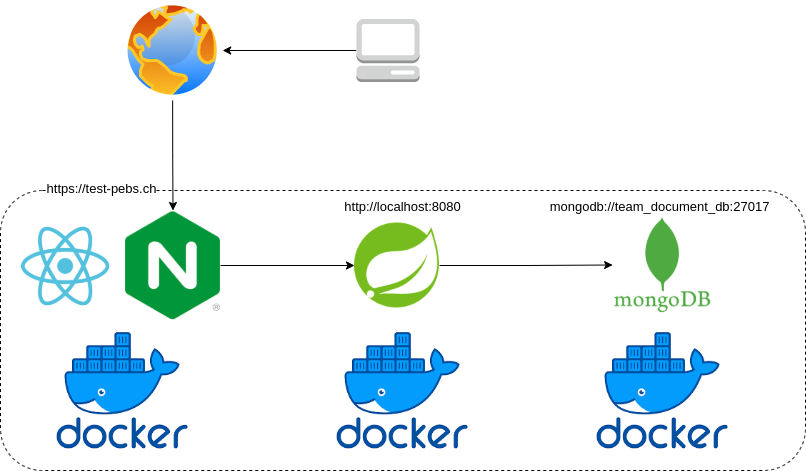
\includegraphics[width=\textwidth,keepaspectratio]{deployment-view}
    \caption{Deployment Übersicht}
    \label{fig:Deplyoment}
\end{figure}
